
\documentclass[11pt,a4paper]{article}
\usepackage{graphicx}
\usepackage{hyperref} 
\author{Computer Engineering: Group 5}
\title{Neural Networks for Medical Diagnosis}
\date{}
\begin{document}
\maketitle

\section{Introduction}
Medicine is a field which records a lot of diagnosis data about the patient, collected through various biological tests, along with final diagnosis.

Artificial Neural Networks (ANNs) will provide a powerful tool to leverage available data to develop predictive models. Such models will help doctors to analyze and make sense of complex clinical data across a broad range of medical applications. Most applications are classification problems; that is, the task is on the basis of the measured features to assign the patient to one of a small set of classes. Their complex structure allows detection of patterns in diagnosis and disease data which might otherwise escape human notice.

Diseases like cancer, diabetes, or certain rare diseases due to malformed genes are difficult to detect in early stages. The results of applying the ANN to diseases based upon selected symptoms show abilities of the network to learn the patterns corresponding to symptoms of the person. Early detection will allow a better, well planned treatment for the patient.

\section{Principle}

The nervous system controls action in humans. It consists mainly of \emph{nerve cells}, called \emph{neurons}. These neurons have electrochemical ion signals as `inputs' and `outputs'. A neuron has a number of \emph{synapses}, which are it's input channels, and an \emph{axon} which is the single output channels. At neuron level, the only decision to be made is this \emph{to fire or not to fire}. Networks of neurons involve \emph{axons} of several neurons `connected' to the \emph{synapses} of others. When the number of inputs firing exceeds a certain value, the neuron \emph{fires}. Out of interaction of several neurons in the network, complex decision making emerges.

This model is used to create artificial neural networks. ANNs can be considered to be a \emph{graph} of \emph{nodes} connected by weighted edges. While real \emph{neurons} can either fire or not fire, in computation, we can instead have a number which represents it's importance in the network. 

\section{Method}
\begin{figure}
	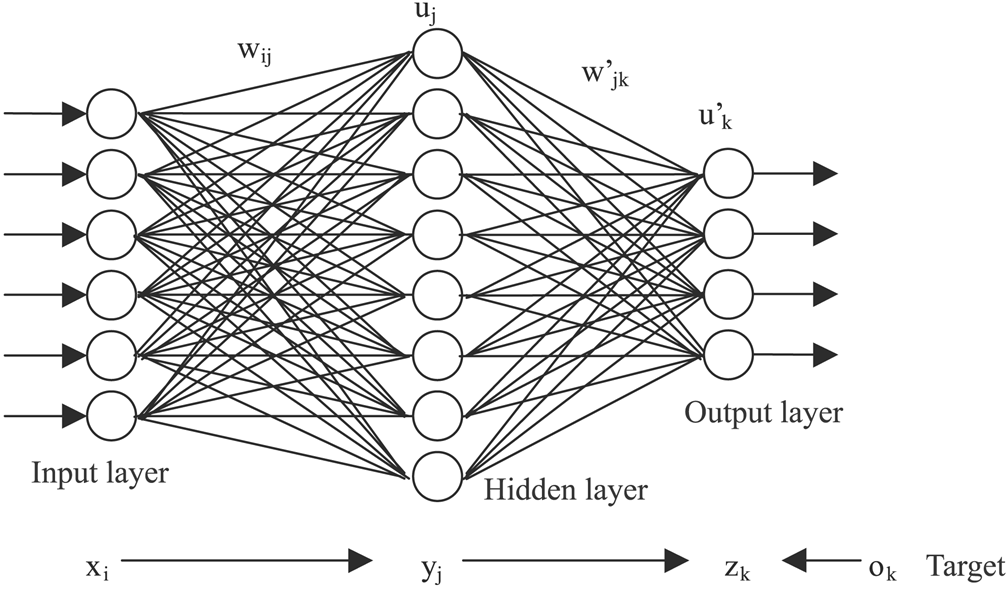
\includegraphics[width=\linewidth]{NeuralNetwork.png}
	\caption{A neural network having a single hidden layer, a 6 dimensional input and a 4 dimensional output}
	\label{fig:network}
\end{figure}
An artificial neural network consists of layers of nodes, each of which holds a value. Groups of node-neurons in each layer fire for specific input patterns, leading to high output values for output neurons corresponding to these patterns.

Now such a node has several inputs from nodes of the previous layer. A weighted sum of these inputs determines the node's activation. These weights correspond to the edge which connects two nodes. The sum represents the \emph{intensity with which the neuron fires} or the \emph{degree} to which it affects the output.

In case a probabilistic model is required a \emph{sigmoid} function, which `compresses' the real line onto the range $ [0, 1] $ is used.

\begin{center}
	$ b = \sigma(w_{1} \cdot a_{1} + w_{2} \cdot a_{2} + \ldots + w_{n} \cdot a_{n}) $
\end{center}


The goal here is to obtain a set of weights for edges in the network, which will cause specific groups of neurons in the network to `fire' for particular inputs, causing corresponding nodes of the output layer to take a higher value.

For example, consider a networks that predicts the chances of cancer based on CT-Scan images. Each pixel in the image will correspond to one dimension of the input vector. Then the weights in a trained network will cause mapping of particular input values that correspond to high chance of cancer to a larger number which indicates a high chance of the disease. Alternately, a network could have multiple outputs which \emph{classify} the cancer into stages. Each output node will correspond to a particular stage, and it's value will represent it's likelihood.

The network will be \emph{trained} by using data for which correct diagnosis is available. This is supervised learning.

An input for which output is known is fed to the network, and the difference between the network's output vector and the known output vector is calculated, \emph{as a function of the weights of the edges}. The \emph{cost} of a particular data point could be considered as the \emph{euclidian distance} between the expected and network outputs. The edge weights are modified in the direction of steepest descent- the direction opposite to the gradient, so as to approach the weights which correspond to the least cost.\cite{3b1b}

A \emph{minima} of this cost function is found, which gives a \emph{trained} network, which has weights adjusted give an outputs that fit into the pattern inherent in the structured data. This \emph{minima} is the set of edge weights which will be used as the \emph{model}\cite{3b1b}

Once the network achieves learning, it can be treated as a \emph{black box} by the final user, which takes `n' inputs and produces `m' outputs.

The advantage of such a method is that it is \emph{not necessary to understand a system} to model it using a neural network. All that is needed is an accurate dataset from which the network can \emph{`learn'}. To the network, what the values represent does not matter, the pattern inherant in the dataset does.

\section{Application}
\begin{figure}
	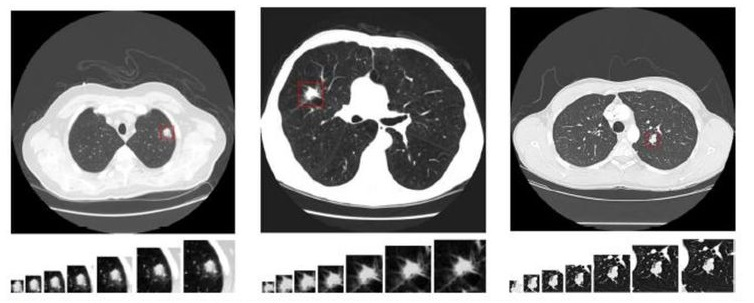
\includegraphics[width=\linewidth]{cnnlung.jpg}
	\caption{CT Examples with lung nodules in different categories. They are benign (left), primary malignant (middle), and metastatic malignant (right).}
	\label{fig:cnn}
\end{figure}

\emph{CNNs} of \emph{Convolutional Neural Networks} are ones which are well suited for processing of image data. In these networks, instead of a \emph{n dimensional vector} the input is an \emph{image} The layers in the network are arranged in such a manner that similarities in characteristics of pixels close together in the image influence the output, whereas those far do not.

Cancer is a disease whose early detection and treatement can greatly improve mortality rates. One method of detection is analysis of images obtained using techniques such as X-Rays, CT-Scans or Magnetic Resonance imaging. Sputum color images can be used for detection of lung cancer. The manual analysis of these images is labourious and time consuming, as also prone to error. False positives are a major problem seen in case of lung cancer screening.\cite{wikipedia} 

There is a lot of image data, along with corresponding case information which is available for use. A data point will consist of a set of images, and final diagnosis and malignancy of cancer. This can be used to develop networks which will provide a preliminary diagnosis of disease based purely on imaging. The network will segment, isolate and then search for patterns which correspond to cancerous tissue, based on patterns recognised in training data.

Researchers at Stanford have developed a network which performs visual diagnosis of skin cancer. The normal process involves naked-eye examination, followed by further examination with a dermatoscope. The network developed for diagnosis of skin lesions matched the performance of actual dermatologists.\cite{skin}

Hopfield Neural networks have been used to extract cytoplasm and nucleus segments from sputum color images, and detect lung cancer. These networks are sensitive even to overlapping cytoplasm classes. \cite{hnn}

Lymph node biopsies are performed for detection of breast cancer. Pathological examination of biopsies is then done for diagnosis. A deep-learning based network has been designed by researchers from CSAIL which process digital whole-slide-images to automatically detect metastatic breast cancer. Their network segment images into tissue, and distinguish tumour patches from normal patches. The network produces a tumour heatmap, which is used to classify the slide image.\cite{csail}

Nowadays, challenges are hosted online by several universities for developing networks with the highest success rate for disease detection, with relevant datasets being provided. Simply based on choice of proper model and training, computer scientists with a minimal biology background can create accurate models. Once trained, such models can be integrated with imaging systems for providing preliminary diagnosis. In case of skin cancers which does not require specialised imaging, mobile phone based applications can be created.\cite{skin}


\section{Conclusion}

ANNs have shown satisfactory diagnosis results in image-based as well as other types of diagnosis. They do not, however surpass humans in accuracy.
Neural networks however offer certain distinct advantages
\begin{itemize}
	\item The ability to process large amount of data
	\item Reduced likelihood of overlooking relevant information
	\item Reduction of diagnosis time
\end{itemize}
\cite{havel}
However, despite their high accuracy rates, they must be considered only as a tool to facilitate the final decision of a clinician, who is ultimately responsible for critical evaluation of the ANN output.

\begin{thebibliography}{99}
\bibitem{havel}Artificial neural networks in medical diagnosis, Journal of Applied Biomedicine
\bibitem{3b1b}Deep Learning, Grant Sanderson \url{https://www.youtube.com/watch?v=aircAruvnKk}
\bibitem{csail}Deep Learning for Identifying Metastatic Breast Cancer \url{https://people.csail.mit.edu/khosla/papers/arxiv2016_Wang.pdf}
\bibitem{skin}Dermatologist-level classification of skin cancer with deep neural networks \url{https://www.nature.com/articles/nature21056}
\bibitem{lung}Deep Convolutional Neural Networks for Lung Cancer Detection \url{http://cs231n.stanford.edu/reports/2017/pdfs/518.pdf}
\bibitem{wikipedia} \url{https://en.wikipedia.org/wiki/Cancer_screening}
\bibitem{hnn}Lung Cancer Detection By Using Artificial Neural Network And Fuzzy Clustering Methods
\end{thebibliography}

\end{document}
